\documentclass[a4paper, 12pt]{article}
\usepackage[utf8]{inputenc}
\usepackage[brazil]{babel}
\usepackage{amstext} 	% need for \text command
\usepackage{amsmath}    % need for subequations
\usepackage{amssymb}
\usepackage{graphicx}   % need for figures
\usepackage{verbatim}   % useful for program listings
\usepackage{color}      % use if color is used in text
\usepackage{subfigure}  % use for side-by-side figures
\usepackage{hyperref}   % use for hypertext links, including those to external documents and URLs
\usepackage{pictexwd}	% use for pictex graphs
\usepackage{booktabs}	% use for Publication quality tables in LaTeX
\usepackage{lipsum}

%\author{Vítor M. Martins}
\title{PME2360}

\begin{document}
\maketitle
%\newpage
%\tableofcontents
%\newpage

\section{Ex. 6}

\begin{figure}[h]
\begin{center}
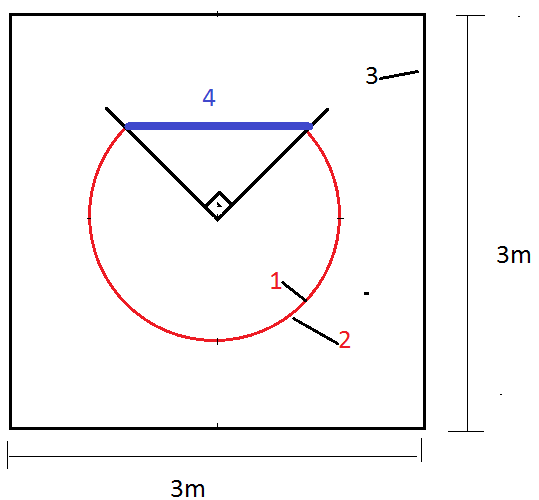
\includegraphics[scale=0.48]{./fig/1.png}
\caption{\label{fig:1}1} 
\end{center}
\end{figure}

\[T_{1} = T_{2} = 1000 \ K\]
\[T_{3} = 300 \ K\]
\[\varepsilon _{3} = \alpha _{3} = 0.2\]

\[\alpha _{3} = 0.2\]
\[\varepsilon _{1} = 0.3\]
\[\varepsilon _{2} = 0.5256\]
\[\alpha _{3} = 0.7180\]

\begin{figure}[h]
\begin{center}
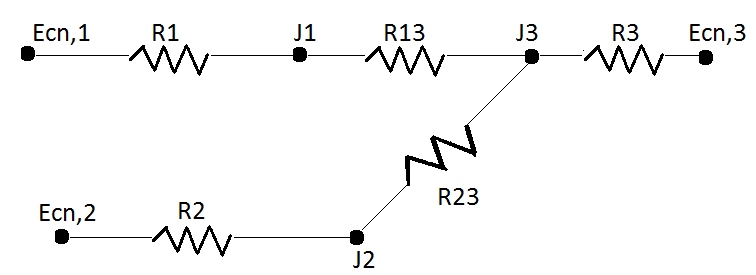
\includegraphics[scale=0.6]{./fig/2.png}
\caption{\label{fig:2}2} 
\end{center}
\end{figure}

\paragraph*{a} $\varepsilon _{2} = ? $
\paragraph*{b} $\alpha _{2} = ? $
\paragraph*{c} $q_{13} = ? $

\[R_{1} = \frac{1-\varepsilon _{1}}{\varepsilon _{1} A_{1}}\]
\[R_{2} = \frac{1-\varepsilon _{2}}{\varepsilon _{2} A_{2}}\]
\[R_{3} = \frac{1-\varepsilon _{3}}{\varepsilon _{3} A_{3}}\]

\[R_{13} = (A_{1}F_{13})^{-1}\]
\[R_{23} = (A_{2}F_{23})^{-1}\]


Superfície difusa: radiação não tem uma direção específica, a superfície emite em todas as direções.

Superfície Cinzenta: emissividade e absorvidade não dependem do comprimento de onda
O exercício tem que dizer que a superfície é cinzenta para podermos montar um circuito, tal como o usado na resolução.

Radiosidade é a contribuiçao líquida da radiação do corpo, e compreende o que o corpo emite e reflete menos o que ele absorve da radiação ambiente. O tipo de resistência que liga as radiosidades num circuito é a geométrica (que tem a ver com o fator de forma). As outras resistências são ditas superficiais, e medem a "distância" $\ $ da radiosidade da superfície do corpo em relação a um corpo negro.

A unidade de radiosidade é $W/m^{2}$. Se a superfície é cinzenta, $\varepsilon = \alpha$

\begin{figure}[h]
\begin{center}
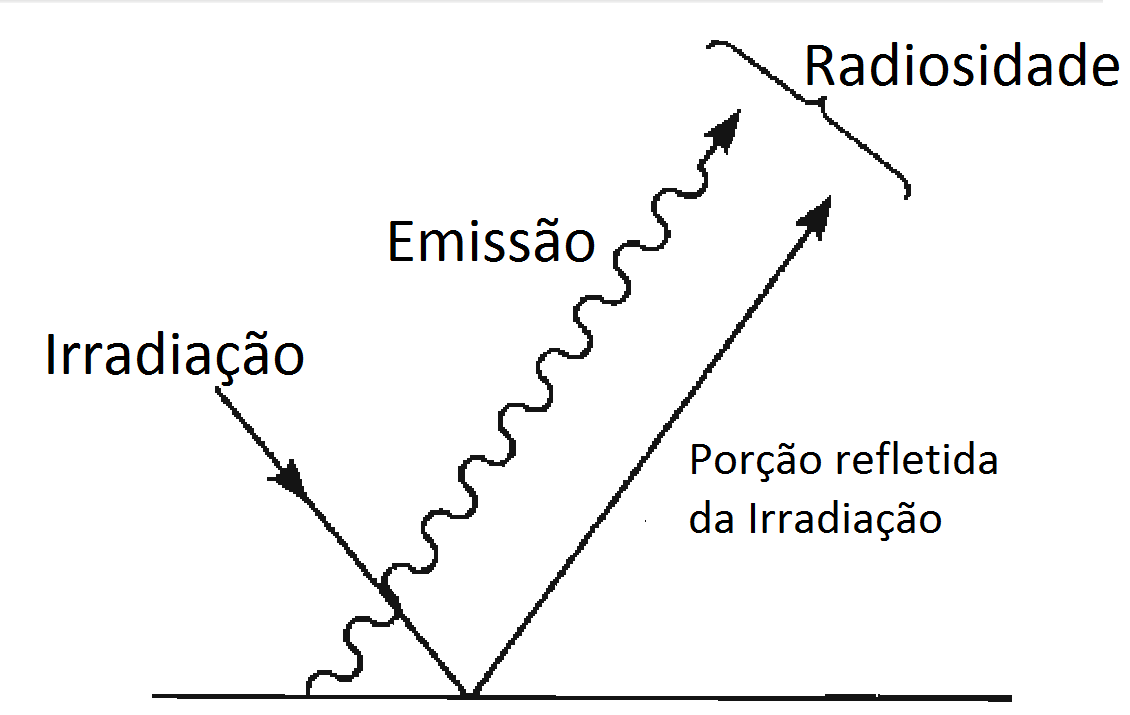
\includegraphics[scale=0.28]{./fig/3.png}
\caption{\label{fig:3}Radiosidade} 
\end{center}
\end{figure}

\[R_{1}' = \frac{1-0.3}{0.3 (2 \pi - \theta )R} = 0.4951 m^{-1}\]
Em que R vale 1 metro
\[R_{2}' = \frac{1-0.5256}{0.5256 (2 \pi - \theta )R} = 0.1914 m^{-1}\]

\[R_{3}' = \frac{1-0.2}{0.2 (2 \pi - \theta )R} = 0.333 m^{-1}\]

\[R_{13} = (0.3 (2 \pi - \theta )R)^{-1} = 0.707 m^{-1}\]
\[R_{23} = (1 (2 \pi - \theta )R)^{-1} = 0.2122 m^{-1} \]

\subsubsection{Cálculo dos Fatores de Forma}
A gente traça uma superfície fictícia, \textit{(4)}, e toda radiaçao que deixa \textit{(1)} e atinge \textit{(4)} também atinge \textit{(3)} (se \textit{(4)} não existisse).
O fator de forma $F_{41}$ = 1 (toda radiaçao que deixa \textit{(4)} (lado de dentro) atinge \textit{(1)})
Logo pela relação de reciprocidade,  
\[A_{4}F_{41} = A_{1}F_{14}\]
Portanto:
\[F_{14} = F_{13} = \frac{A_{4}}{A_{1}} F_{41}\]
Em que $F_{41}$ vale 1. 
\[F_{13} = \frac{2R\sin(\pi / 4) }{(2 \pi - \theta )R}\]
Em que $\theta$ vale $\pi /2$
 
$F_{23}$ = 1  (toda a radiação que deixa \textit{(2)} atinge \textit{(3)} $\rightarrow$ \textit{(2)} não pode atingir ela mesma)

\subsubsection{Soluçao do circuito}


\begin{itemize}
\item $q_{13}$ é a corrente que sai de $E_{CN,1}$ e chega em $J_{3}$
\item $q_{23}$ é a corrente que sai de $E_{CN,2}$ e chega em $J_{3}$
\item $q_{3}$ é a corrente que sai de $J_{3}$ e chega em $E_{CN,3}$
\end{itemize}

\[q_{13}' = \frac{E_{CN,1}-J_{3}}{R_{1}'+R_{13}'} = 0.8318(56690-J_{3})\]
Com $E_{CN,1}$ = $\sigma T_{1}^{4}$

\[q_{23}' = \frac{E_{CN,2}-J_{3}}{R_{2}'+R_{23}'} = 2.480(56690-J_{3})\]

\[q_{3}' = \frac{-E_{CN,3}+J_{3}}{R_{3}'} = 3.003(-459.19+J_{3})\]
Em que $E_{CN,3}$ = $\sigma T_{3}^{4}$

\[q_{3}'=q_{13}'+q_{23}'\]

\[J_{3} = 29949 \ W/m^{2}\]
\[q_{3}' = 88559 \ W/m (d)\]
\[q_{23}' = 66317 \ W/m \]
\[q_{13}' = 22243 \ W/m (c)\]

\subsection{E)}
$T_{2} = T_{1} = ? $ para $q_{3}$`= $2\times q_{3}'$ (item d) = $2 \times 88559$ = $177118 \ W/m$

\[\varepsilon _{2} = 0.2F_{0 \rightarrow 1} + 0.5(F_{0 \rightarrow 10}-F_{0 \rightarrow 1}) 0.8(1-F_{0 \rightarrow 10})\] 

Para T = 1000 K
\begin{itemize}
\item $F_{0 \rightarrow 10}$ = 0.914199
\item $F_{0 \rightarrow 1}$ = 0.000321
\end{itemize}

Para a nova temperatura, $F_{0 \rightarrow 10}$ (novo) $>$ $F_{0 \rightarrow 10}$ 
Hipótese: $F_{0 \rightarrow 10}$ (novo) = 1, portanto $\varepsilon _{2}^{(1)}$ = 0.5.

$F_{0 \rightarrow 1}$ = 0

\[177118 = 3.003(J_{3}-459.19)\]
\[q_{23}'=2.3562(E_{CN,1}-59439)\]
Em que $E_{CN,2}$ = $\sigma T_{1}^{4}$
\[q_{13}'=0.8318(E_{CN,1}-59439)\]

\[T_{1}^{1}=1193K\]


% \begin{center}
%  \fbox{\input{latex2d}}
%  \end{center}



\[F_{0 \rightarrow 10} = 0.944378\]
\[F_{0 \rightarrow 1} = 0.002070\]

\[\varepsilon _{2}^{2} = 0.5173\]
\[T_{1}^{(2)}=1190 \ K\]

\[\varepsilon _{2}^{3} = \varepsilon _{2}^{2}\]

A gente duplicou a potência mas não sabemos qual a nova temperatura. Então, para resolver o item \textbf{e)}, só trocamos os potenciais e algumas resistências do circuito anterior. Nenhuma resistência geométrica mudou, apenas a da emissividade 2. Então o formato do circuito anterior continua válido, só que agora com as trocas dos valores de potenciais e resistências. 

Não sabemos os poderes emissivos dos corpos negros, mas sabemos $q_{13}$. Os potenciais são diferentes, e agora tenho que estimar os valores de emissividade. Temos que chutar uma emissividade. Achamos os valores de temperatura, achamos os valores de fração em cada banda, e então achamos a emissividade, e conferimos se bate com a emissividade chutada inicialmente.

\section{Trocadores de calor}
Calculos de trocador de calor, serve para (dado um trocador de calor), calcular as temperaturas na saída do trocador de calor, ou, dada uma temperatura final, determinar as dimensões desse trocador de calor.

O papel das chicanas é aumentar a superfície no interior do casco.

Trocadores de calor compactos tem áreas extremamente elevadas para volumes pequenos.
O fluido passa por passagens extremamente extensas e finas, com escoamento laminar.

\end{document}